\begin{figure}[htb]
    \centering
    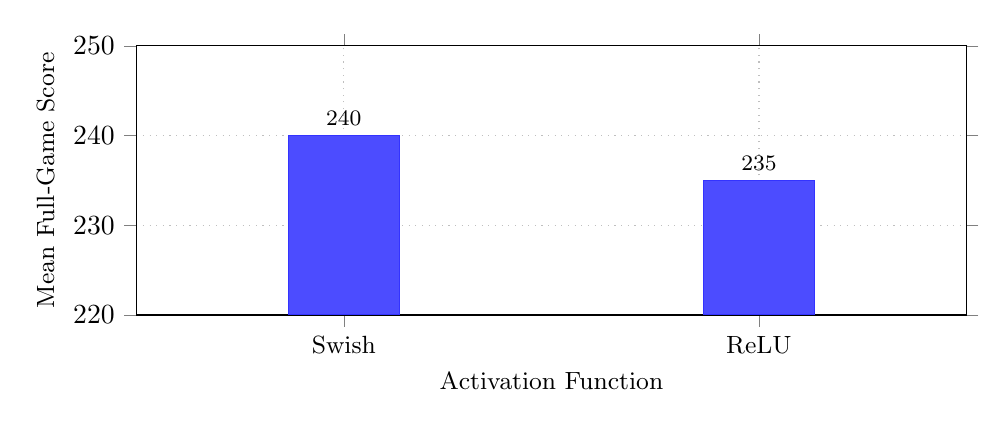
\begin{tikzpicture}
        \begin{axis}[
                ybar,
                width=\columnwidth,
                height=5cm,
                xlabel={Activation Function},
                ylabel={Mean Full-Game Score},
                symbolic x coords={Swish, ReLU},
                xtick=data,
                xticklabel style={font=\small},
                ylabel style={font=\small},
                xlabel style={font=\small},
                bar width=40pt,
                ymin=220, ymax=250,
                grid=both,
                grid style={dotted},
                tick align=outside,
                nodes near coords,
                nodes near coords style={font=\footnotesize, anchor=south},
                enlarge x limits=0.5,
            ]

            \addplot[
                fill=blue!70!white,
                draw=blue!80,
                error bars/.cd,
                y dir=both,
                y explicit
            ] coordinates {
                    (Swish, 240)
                    (ReLU, 235)
                };

        \end{axis}
    \end{tikzpicture}
    \caption{Performance comparison: Swish vs ReLU activation (placeholder data)}
    \label{fig:silu-vs-relu}
\end{figure}
